%
% ======================================================================
\RequirePackage{docswitch}
% \flag is set by the user, through the makefile:
%    make note
%    make apj
% etc.
\setjournal{\flag}

\documentclass[\docopts]{\docclass}

% You could also define the document class directly
%\documentclass[]{emulateapj}

% Custom commands from LSST DESC, see texmf/styles/lsstdesc_macros.sty
\usepackage{lsstdesc_macros}

\usepackage{graphicx}
\graphicspath{{./}{./figures/}}
\bibliographystyle{apj}

% Add your own macros here:



%
% ======================================================================

\begin{document}

\title{ The LSST DESC Data Challenge 1: Simulating data for the next generation of photometric redshift surveys }

\maketitlepre

\begin{abstract}

The success of future Stage IV dark energy surveys~\citep{2006astro.ph..9591A} relies in the ability to model and mitigate
systematic uncertainties. Realistic simulation offer a unique opportunity to study systematic uncertainties and test the
processing and analysis pipelines of ongoing and future experiments. Here we present a set of realistic simulations
of $\sim 40$ sq.-deg. that try to mimic the depth and characteristics of LSST 10-years coadd images in the $r$-band.
We characterize our samples performing several astrometric and photometric checks to assess the quality of the
measurements and to enable the usage of these simulations for future studies.

\end{abstract}

% Keywords are ignored in the LSST DESC Note style:
\dockeys{latex: templates, papers: awesome}

\maketitlepost

% ----------------------------------------------------------------------
%

\section{Introduction}
\label{sec:intro}

The increase in statistical power from recent cosmological experiments makes the modeling, and mitigation of systematic
uncertainties key to extract the maximum performance and produce competitive analyses. More traditional in high energy
particle physics~\citep{Brun:118715},~\citep{2006JHEP...05..026S}, end-to-end simulations provide a unique framework to
model systematics and streamline processing and analysis pipelines given that we have complete information about the inputs
and outputs. With the larger availability of computational resources this approach has also been extended to photometric
redshift galaxy surveys~\citep{2016MNRAS.457..786S,2016ApJ...817...25B} and a similar effort is undergoing in spectroscopic
surveys such as DESI~\citep{2016arXiv161100036D}. For surveys like the LSST~\citep{2008arXiv0805.2366I} where the expected
data volume is very large and where a highly stringent control of the systematic uncertainties is required, producing these
kind of end-to-end simulations becomes necessary.

In this paper, we present the procedure to generate and process images that resemble the data that will be produced by
LSST~\citep{2008arXiv0805.2366I} after 10 years of operation in $r$-band using state of the art tools. We also characterize
the products of this process for future studies. These productsencompass single-visit and coadded calibrated exposures
(i.e., flattened, background removed, etc) and source catalogs that add up to $\sim 225 TB$. They are the result of three
different simulations: imSim dithered, imSim undithered, and PhoSim that will be introduced later.

This paper is structured as follows: In Section \secref{inputs} we describe the input catalog used for our simulations,
in Section \secref{image_generation_pipeline} we introduce two different approaches to generate simulated images to
resemble LSST data. In Section \secref{image_processing_pipeline} we present the procedure and tools used to perform
calibration and source extraction on the simulated images. In Section \secref{catalogs} we describe the output catalogs
produced by our pipelines. Finally, in Section \secref{conclusions} we present some concluding remarks.

% ----------------------------------------------------------------------
\section{Image generation: inputs}
\label{sec:inputs}

\textcolor{red}{Describe CatSim inputs and dithering}

\section{Image generation: pipeline}
\label{sec:image_generation_pipeline}
% ---------------------------------------------------------------------

The artificial generation of astronomical images is a very complex and computationally demanding process. In the recent
years there is a big effort in the community in order to create software that allows more realistic and fast image
generation~\citep{2016MNRAS.457..786S,2016ApJ...817...25B}. In our case, we use two different approaches: In one approach
we use modeling of the input sources using \textsc{GalSim}~\citep{2015A&C....10..121R}. The other approach consists in
running a full photon-shooting simulation using \textsc{PhoSim}~\citep{2015ApJS..218...14P}. The former has a big speed
advantage but the latter fully traces each photon coming from the sources through the atmosphere and the instrument,
 increasing the level of realism. These two approaches allow us to focus on different systematic effects and science cases.

\subsection{The imSim pipeline}
\label{sec:imsim_pipeline}

\textcolor{red}{Describe imSim}
% ----------------------------------------------------------------------

\subsection{The PhoSim pipeline}
\label{sec:phosim_pipeline}

\textcolor{red}{Describe PhoSim}
% ----------------------------------------------------------------------

\section{Image processing pipeline}
\label{sec:image_processing_pipeline}

Once the images are produced we process them using the LSST software stack~\citep{2015arXiv151207914J}. This is an open
source high-performance data processing and analysis system intended for use in O/IR survey data. The code can be found at
\url{dm.lsst.org} and \url{pipelines.lsst.io}. The raw, uncalibrated single exposures are used as inputs. The software performs
the reduction, detection, deblending and measurement on individual visits and coadds producing the level 2 data
products~\citep{2015arXiv151207914J}.

\textcolor{red}{Say something about data size, times, configuration, etc}
% ----------------------------------------------------------------------

\section{Output catalogs}
\label{sec:catalogs}

After being processed, the catalogs are accessible by DESC collaborators andstored at NERSC. We generate pandas
dataframes and three different databases for each one of the total coadd catalogs in order to be accessed by the
collaborators and perform their own analyses. These catalogs contain 10.6 million objects covering an area
of $\sim$ 43 deg$^{2}$.

In order to check the level of realism and the accuracy of the processed catalogs we perform several quality assurance tests.
We focus on three different areas that can induce a systematic effect in the weak lensing and clustering observables:
astrometry, photometry and PSF.

\subsection{Astrometry checks}
\label{sec:astrometry_checks}

Biases on astrometry can potentially affect both clustering and weak lensing measurements. These biases
can have different origins: PSF mis-characterization, not corrected sensor effects, presence of blended sources are among
the most common scenarios for single-visit exposures. In the case of co-adds we should add to this list a different effect:
incorrect modeling of proper motion for the measured objects.

We will follow two approaches to check the quality of the astrometric solutions that we obtained: an \textit{external} check
comparing to the input \textit{truth} catalog; and an \textit{internal} check comparing different visits.

\subsubsection{External checks}
\label{sec:external_astrometry}

As we have already mentioned, one of the big advantages of using simulations is that we have access to the \textit{true}
underlying information. We will use this information to check the precision of the astrometric measurements in single exposures
and co-adds. In both cases we will use a \texttt{KDTree}~\citep{scikit-learn} to retrieve those objects in the input catalog
that are in a radius of 0.2 arc-seconds of those detected in the output catalog and select the match that is closest in
magnitude. We only consider sources which have a magnitude difference smaller than 0.05 magnitudes.

We selected a representative single visit and calculated the difference between the measured and the input positions.
These are represented in Figure~\figref{astrometry_a}. We can see that both RA and Dec distributions are compatible with each
other, meaning that there are no anisotropies in the detection, as expected from the inputs. However, we find that the distributions
are assymetric and that the median is not zero. This effect is even more noticeable when we accumulate all of the visits and
it is present in the dithered and undithered runs.

\begin{figure}
  \centering
  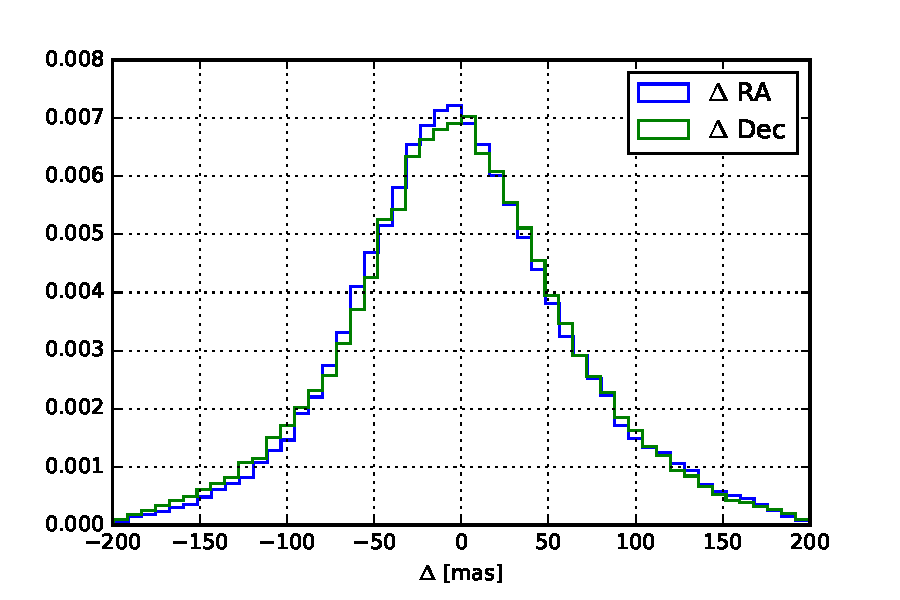
\includegraphics[width=0.45\textwidth]{astrometry_single_visit_imsim_dithered_hist}
  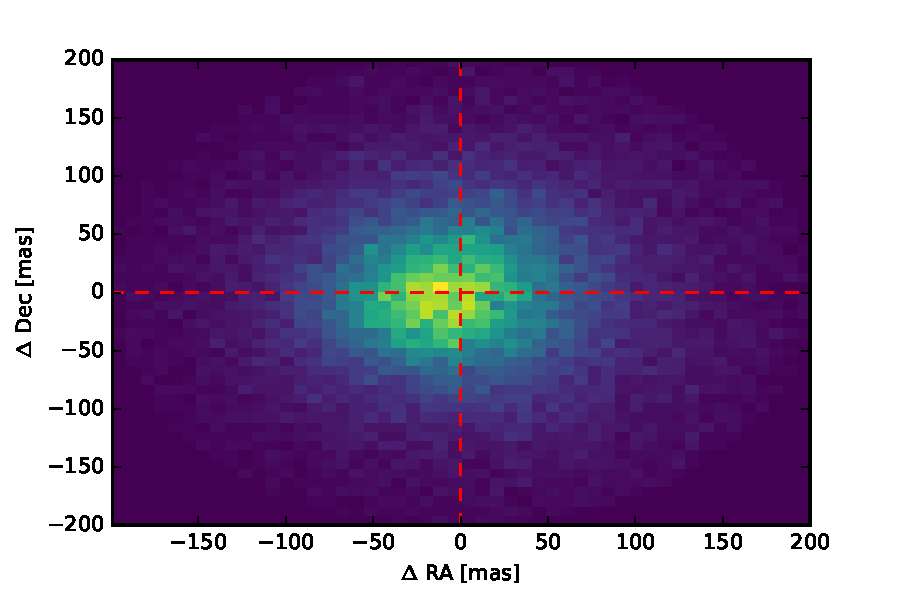
\includegraphics[width=0.45\textwidth]{astrometry_single_visit_imsim_dithered_hist2d}
  \caption{Distribution of the difference $\Delta=X_{measured}-X_{input}$ in RA (blue) and Dec (green) coordinates. We cannot
  appreciate any differences between these, however we see that there is median is not at zero $\Delta_{median} \approx -2$ mas.
  The histograms are normalized such that the total sum of the counts is equal to one. We selected one random representative
  exposure (visit number $270675$ for the \textsc{imSim} dithered run).}
  \label{fig:astrometry_a}
\end{figure}
\subsubsection{Internal checks}
\label{sec:internal_astrometry}

For the internal checks we select two
\subsection{Photometry checks}
\label{sec:photometry_checks}

\subsection{PSF checks}
\label{sec:psf_checks}

% ----------------------------------------------------------------------

\section{Conclusions}
\label{sec:conclusions}


% ----------------------------------------------------------------------

\subsection*{Acknowledgments}

Here is where you should add your specific acknowledgments, remembering that some standard thanks will be added
via the \code{acknowledgments.tex} and \code{contributions.tex} files.

% 
This is the text imported from \code{acknowledgments.tex}, and will be replaced by some standard LSST DESC boilerplate at some point.
% 


Author contributions are listed below. \\
Yusra AlSayyad: Contribution \\
Humna Awan: Contribution \\
Colin Burke: Contribution \\
Jun Cheng: Contribution \\
James C. Chiang: Contribution \\
Scott Daniel: Contribution \\
Seth Digel: Contribution \\
Richard Dubois: Contribution \\
Eric Gawiser: Contribution \\
Tom Glanzman: Contribution \\
Mike Jarvis: Contribution \\
Tony Johnson: Contribution \\
Heather Kelly: Contribution \\
David Kirkby: Contribution \\
Simon Krughoff: Contribution \\
Robert Lupton: Contribution \\
Rachel Mandelbaum: Contribution \\
P.~Marshall: Contribution \\
Mustafa Mustafa: Contribution \\
En-Hsin Peng: Contribution \\
John Peterson: Contribution \\
Paul Price: Contribution \\
Javier Sanchez: Validation and analysis, started note \\
Glenn Sembroski: Contribution \\
Anze Slosar: Contribution \\
Brian Van Klaveren: Contribution \\
Chris W. Walter: Contribution \\
Matt Wiesener: Contribution \\
Bo Xin: Contribution \\


%{\it Facilities:} \facility{LSST}

% Include both collaboration papers and external citations:
\bibliography{lsstdesc,main}

\end{document}
% ======================================================================
%
